\chapter{Análisis del rendimiento de procesos contenerizados}

Para comprobar cómo de factible es la idea de la ejecución de procesos de tiempo
real virtualizados mediante contenedores, hemos llevado a cabo una serie de
pruebas con el objetivo de caracterizar algunos aspectos de su funcionamiento.
Todas las pruebas han sido realizadas sobre el dispositivo Raspberry Pi
detallado en la sección \ref{sec:01-tools}. Se ha hecho uso de la suite de
pruebas \texttt{rt-tests}, la cuál contiene múltiples utilidades para obtener
métricas sobre el rendimiento del kernel de Linux relevantes en entornos de
tiempo real. Dentro de todas las pruebas posibles que contiene
\texttt{rt-tests}, \texttt{cyclicdeadline} ha sido la utilizada. Esta prueba,
derivada del conocido \texttt{cyclictest}, mide la latencia en la activación de
tareas de tiempo real, es decir, la diferencia de tiempo entre el momento en el
que se debería activar una tarea y en el que se activa realmente. La principal
diferencia entre \texttt{cyclictest} y \texttt{cyclicdeadline} reside en que la
primera mide la latencia para tareas planificadas con \texttt{SCHED\_FIFO}
(planificación estática), mientras que la segunda hace lo propio con
\texttt{SCHED\_DEADLINE}. Como se ha indicado en la sección
\ref{sec:02-real_time}, esta última es la política de planificación elegida para
el sistema que se desea desarrollar, razón por la cuál hemos decidido usar
\texttt{cyclicdeadline}.

Concretamente, se han hecho varias ejecuciones de esta prueba aumentando cada
vez el número de hilos de tiempo real que se debían ejecutar y observar. Para
todos los hilos, el límite de tiempo o \textit{deadline} ha sido de 1000$\mu s$.
Estas pruebas se han realizado dos veces: primero, ejecutando
\texttt{cyclicdeadline} de forma «nativa» y, luego, dentro de un contenedor. La
definición de la imagen Docker que contiene la prueba, así como los pasos
seguidos para su ejecución, son explicados detalladamente en el apéndice
\ref{app:03-container_tests}. Los resultados obtenidos son los mostrados en la
tabla \ref{tab:03-cyclicdeadline_latency}. Cabe destacar que
\texttt{cyclicdeadline} solo nos devuelve al final de su ejecución, para cada
uno de los hilos, los valores mínimo, máximo y medio de la latencia. Por ello,
los resultados de la tabla para ejecuciones con más de un hilo muestran
realmente el mínimo de los mínimos de los hilos, el máximo de los máximos y la
media de las medias.

\begin{table}
    \centering
    \begin{tabular}{ | c | c | c | c | c | }
        \hline
                      &                & \textbf{Latencia}         & \textbf{Latencia}         & \textbf{Latencia}        \\
        \textbf{Tipo} & \textbf{Hilos} & \textbf{mínima ($\mu s$)} & \textbf{máxima ($\mu s$)} & \textbf{media ($\mu s$)} \\
        \hline
        Contenedor    & 1              & 1                         & 113                       & 22.0                     \\
        \hline
        Contenedor    & 2              & 1                         & 257                       & 85.0                     \\
        \hline
        Contenedor    & 3              & 1                         & 362                       & 127.33                   \\
        \hline
        Contenedor    & 4              & 1                         & 426                       & 112.0                    \\
        \hline
        Contenedor    & 5              & 1                         & 527                       & 210.20                   \\
        \hline
        Contenedor    & 6              & 1                         & 700                       & 263.0                    \\
        \hline
        Nativo        & 1              & 1                         & 88                        & 17.0                     \\
        \hline
        Nativo        & 2              & 1                         & 267                       & 123.0                    \\
        \hline
        Nativo        & 3              & 1                         & 332                       & 149.0                    \\
        \hline
        Nativo        & 4              & 1                         & 307                       & 122.0                    \\
        \hline
        Nativo        & 5              & 3                         & 448                       & 196.0                    \\
        \hline
        Nativo        & 6              & 1                         & 613                       & 205.67                   \\
        \hline
    \end{tabular}
    \caption{Resultados obtenidos de la ejecución de \texttt{cyclicdeadline}.}
    \label{tab:03-cyclicdeadline_latency}
\end{table}

Lo que queríamos observar con estas pruebas es el impacto que tiene sobre la
latencia el uso de Docker. En la gráfica de la figura
\ref{fig:03-cyclicdeadline_latency}, se muestran los datos de la anterior tabla
de forma que este impacto se hace evidente. Aunque la latencia media se mantiene
relativamente similar, el límite superior es mayor en las ejecuciones
contenerizadas. No obstante, el impacto no es especialmente notable, de forma
que se puede seguir considerando como una herramienta factible para el
despliegue de procesos de tiempo real, si bien no será recomendable para los que
tengan unas restricciones temporales más pequeñas donde esta latencia sea
demasiado alta.

\begin{figure}
    \centering
    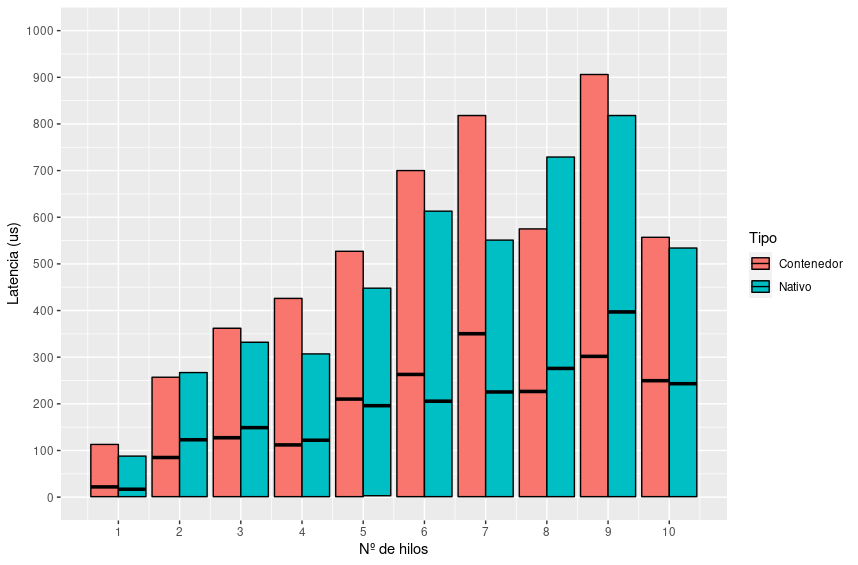
\includegraphics[width=\textwidth]{03-container_analysis/cyclicdeadline-latency.png}
    \caption{Gráfica de intervalos con los rangos de latencia mínima a máxima
        obtenidos de la ejecución de \texttt{cyclicdeadline}. Para cada rango, se
        muestra también su media.}
    \label{fig:03-cyclicdeadline_latency}
\end{figure}

Hay que tener en cuenta que la ejecución de \texttt{cyclicdeadline} dentro de un
contenedor se realiza de forma que este programa lanza los hilos de tiempo real
dentro de su mismo contenedor, el cuál ya se encuentra en ejecución. Por ello,
se decidió realizar una segunda prueba con el objetivo de analizar la latencia
en el lanzamiento de los propios contenedores, dato que es especialmente
importante en el contexto que se plantea para la herramienta de orquestación de
tareas de tiempo real, dado que estas tareas se deben lanzar en los nodos desde
cero. Para que la ejecución del proceso de prueba no influya en los resultados,
se ejecuta todo este proceso desde un ordenador externo «maestro». El
funcionamiento es el siguiente:

\begin{enumerate}
    \item El maestro lanza un contenedor en la Raspberry Pi mediante SSH.
    \item Cuando el contenedor se lanza, envía un mensaje UDP de vuelta al
          maestro informando de que ha terminado su ejecución.
    \item El maestro obtiene los tiempos de creación e inicio del contenedor
          ejecutando el comando \texttt{docker inspect} mediante SSH.
    \item La latencia se obtiene como la diferencia entre ambos tiempos.
    \item El maestro elimina el contenedor de la Raspberry Pi mediante SSH para
          poder lanzarlo de nuevo en la siguiente iteración.
\end{enumerate}

Para comprobar también si el lenguaje usado en la implementación del proceso
contenerizado tiene algún impacto sobre esta latencia, se han usado tres
versiones diferentes del contenedor que se lanza sobre la Raspberry Pi, usando
C, Go y Rust. Los tres son lenguajes compilados con similitudes en cuanto a su
alcance (programación de sistemas) y características. En total, se han realizado
1000 iteraciones de esta prueba para cada uno de los lenguajes. Los resultados
obtenidos se muestran en la tabla \ref{tab:03-container_latency}. En la figura
\ref{fig:03-container_latency} se puede observar una representación gráfica de
todas las latencias observadas para cada iteración.

A primera vista, apreciamos que el lenguaje usado para la implementación de los
procesos contenerizados no tiene ningún impacto sobre la latencia en su
lanzamiento. Por otro lado, se trata de valores muy altos, demasiado como para
que podamos considerar el lanzamiento de un contenedor como parte de una tarea
de control dura. También destaca la gran variación de estas latencias. Todo esto
nos hace pensar que la implementación que tiene Docker de sus tareas de gestión
del ciclo de vida de los contenedores no están preparadas para ser
deterministas, aunque, obviamente, dudamos de que este aspecto fuera considerado
en su diseño.

\begin{table}
    \centering
    \begin{tabular}{ |c|c|c|c|c| }
        \hline
                          & \textbf{Tiempo}        & \textbf{Tiempo}        & \textbf{Tiempo}       & \textbf{Desviación} \\
        \textbf{Lenguaje} & \textbf{mínimo ($ms$)} & \textbf{máximo ($ms$)} & \textbf{medio ($ms$)} & \textbf{típica}     \\
        \hline
        C                 & 1472                   & 2548                   & 1693                  & 165                 \\
        \hline
        Go                & 1445                   & 2718                   & 1693                  & 163                 \\
        \hline
        Rust              & 1478                   & 2378                   & 1701                  & 156                 \\
        \hline
    \end{tabular}
    \caption{Valores observados para la latencia en el lanzamiento de
        contenedores implementados en distintos lenguajes.}
    \label{tab:03-container_latency}
\end{table}


\begin{figure}
    \centering
    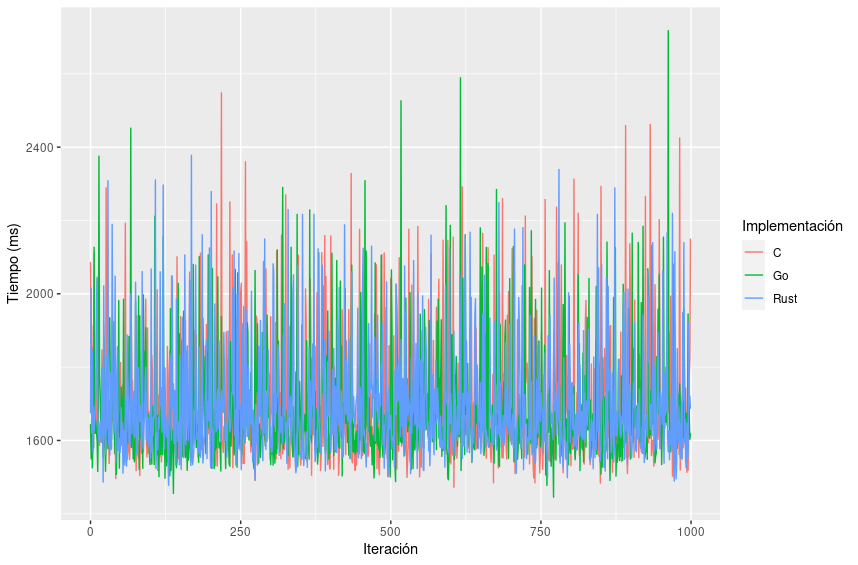
\includegraphics[width=\textwidth]{03-container_analysis/container-latency.png}
    \caption{Gráfico de líneas con las latencias observadas en el lanzamiento de
        contenedores implementados con distintos lenguajes.}
    \label{fig:03-container_latency}
\end{figure}